\chapter{Sentencepiece default parameters}


\begin{table}[h]
    \centering
    \begin{tabular}{|p{5.3cm}|p{5cm}|p{2cm}|}
    \hline
    \textbf{Parameter Name} & \textbf{Explanation} & \textbf{Default} \\
    \hline
    \textbf{model\_type} & Model algorithm: unigram, bpe, word, or char & "unigram" \\
    \hline
    \textbf{vocab\_size} & Vocabulary size & 8000 \\
    \hline
    \textbf{character\_coverage} & Character coverage to determine the minimum symbols & 0.9995 \\
    \hline
    \textbf{input\_sentence\_size} & Maximum size of sentences the trainer loads & 0 \\
    \hline
    seed\_sentencepiece\_size & The size of seed sentencepieces & 1000000 \\
    \hline
    shrinking\_factor & Keeps top shrinking\_factor pieces with respect to the loss & 0.75 \\
    \hline
    num\_sub\_iterations & Number of EM sub-iterations & 2 \\
    \hline
    max\_sentencepiece\_length & Maximum length of sentence piece & 16 \\
    \hline
    max\_sentence\_length & Maximum length of sentence in byte & 4192 \\
    % \hline
    % split\_by\_unicode\_script & Use Unicode script to split sentence pieces & true \\
    % \hline
    % split\_by\_number & Split tokens by numbers (0-9) & true \\
    % \hline
    % split\_by\_whitespace & Use a white space to split sentence pieces & true \\
    % \hline
    % split\_digits & Split all digits (0-9) into separate pieces & false \\
    % \hline
    % treat\_whitespace\_as\_suffix & Treat whitespace marker as suffix instead of prefix & false \\
    % \hline
    % allow\_whitespace\_only\_pieces & Allow pieces that only contain (consecutive) whitespace tokens & false \\
    % \hline
    % normalization\_rule\_name & Normalization rule name. Choose from nfkc or identity & "nmt\_nfkc" \\
    % \hline
    % remove\_extra\_whitespaces & Removes leading, trailing, and duplicate internal whitespace & true \\
    \hline
    \end{tabular}
    \caption{Default parameters for Sentencepiece training. We bold the parameters that we modify in some of our experiments. Summarized from \url{https://github.com/google/sentencepiece/blob/master/doc/options.md}}
    \label{tab:sentencepiece_defaults}
\end{table}
    

% \chapter{Distances between languages}

% \begin{figure}[h]
%     \centering
%     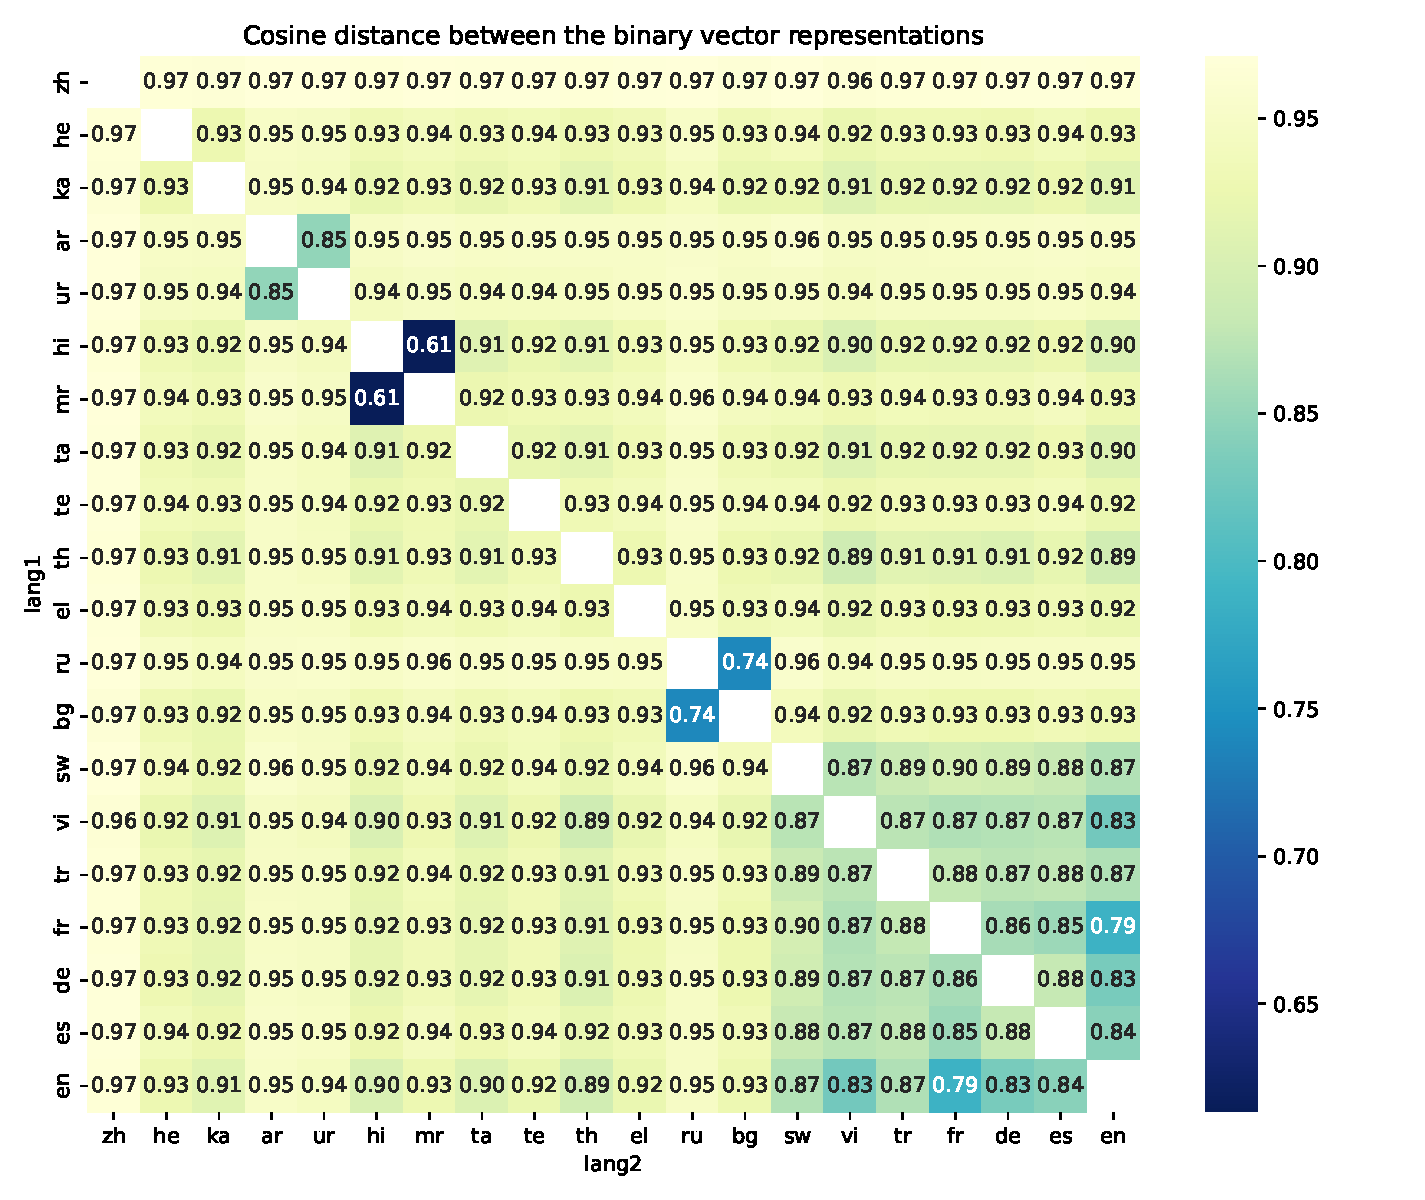
\includegraphics[width=\textwidth]{figures/chung_distances.pdf}
%     \caption{Cosine distances between the language vectors $\vec{v}^l$ for Chung et al.}
%     \label{fig:chung_distances}
% \end{figure}

% % \begin{figure}[h]
% %     \centering
% %     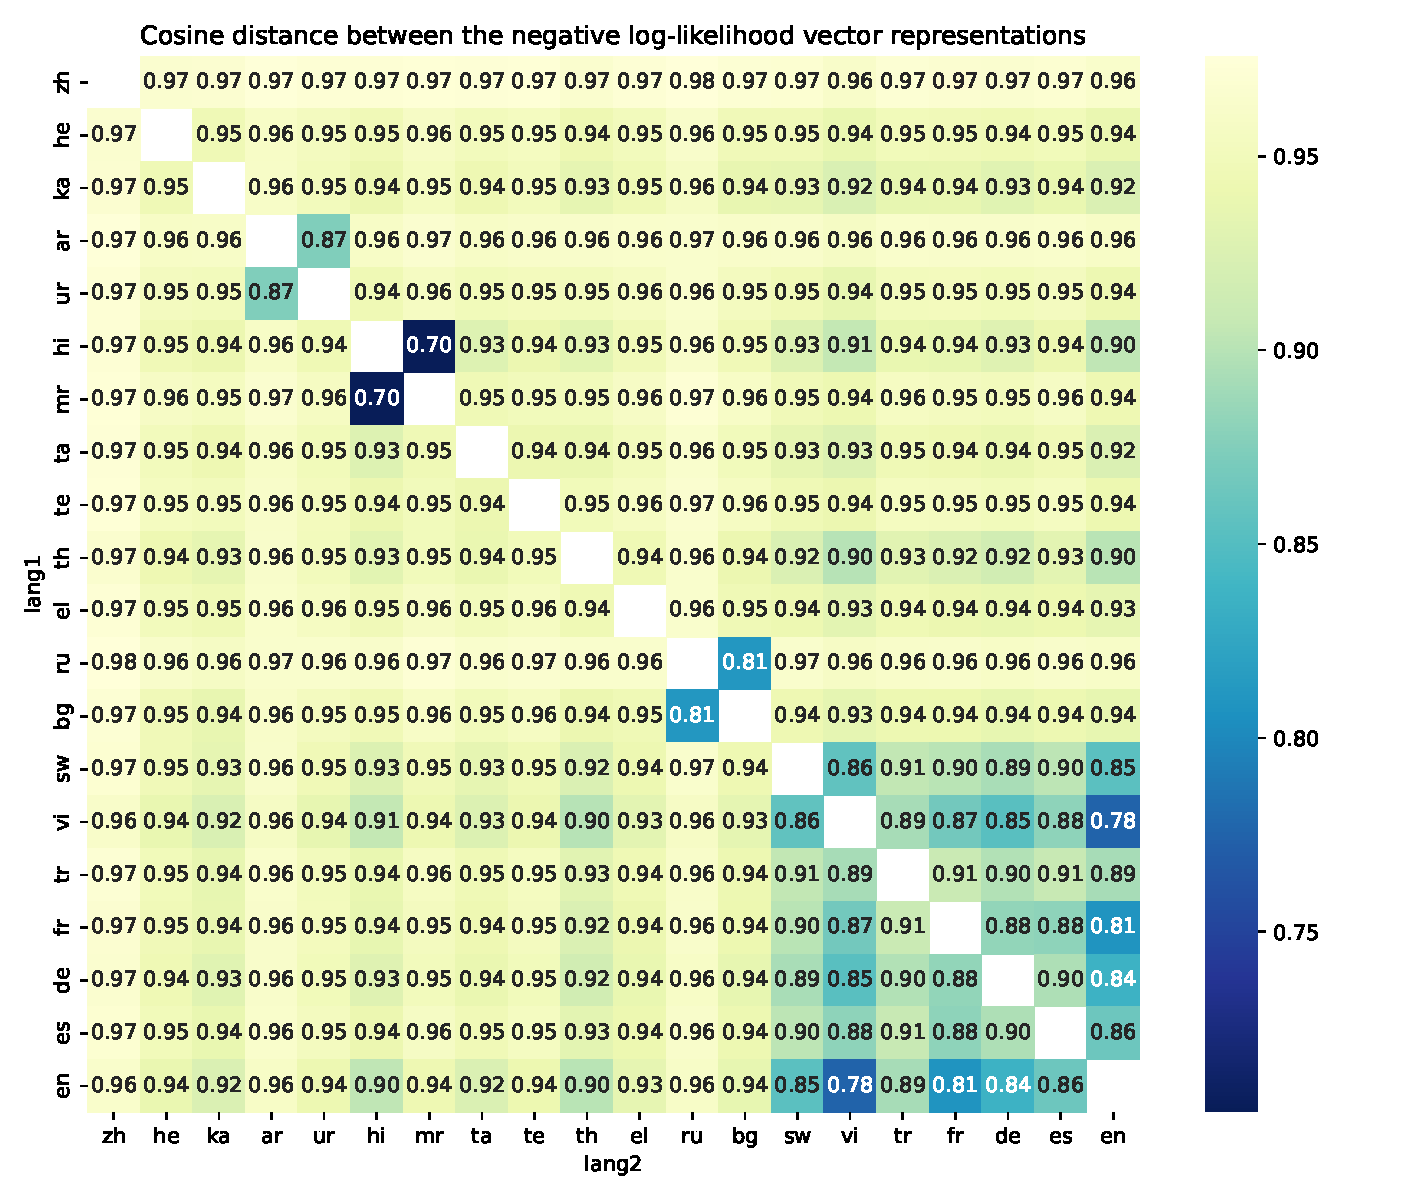
\includegraphics[width=\textwidth]{figures/liang_cosine_distances.pdf}
% %     \caption{Cosine distances between the language vectors $\vec{v}^l$ for Liang et al.}
% %     \label{fig:liang_cosine_distances}
% % \end{figure}

% \begin{figure}[h]
%     \centering
%     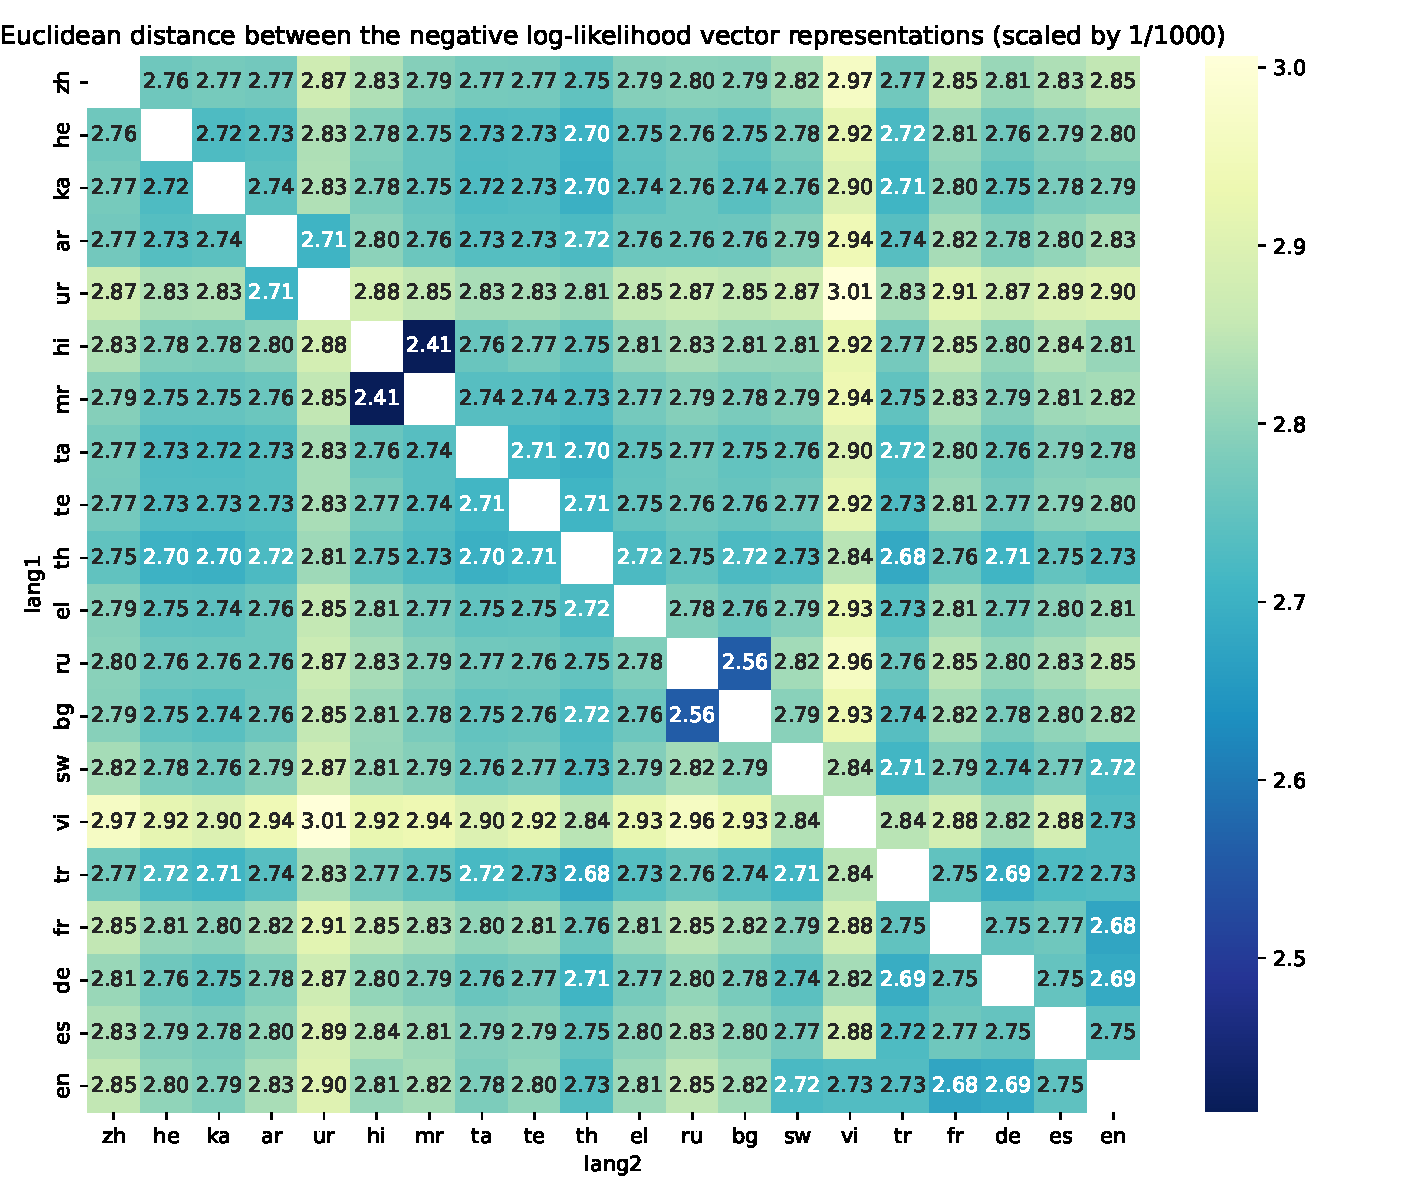
\includegraphics[width=\textwidth]{figures/liang_euclid_distances.pdf}
%     \caption{Euclidean distances between the language vectors $\vec{v}^l$ for Liang et al.}
%     \label{fig:liang_euclid_distances}
% \end{figure}
